\section{Surface Parameterization Methods}
\label{sec:Surface-Parameterization-Methods}

This \cgal\ package implements some of the state-of-the-art
surface parameterization methods, such as Least Squares Conformal Maps,
Discrete Conformal Map, Discrete Authalic
Parameterization, Floater Mean Value Coordinates or Tutte Barycentric
Mapping. These methods are provided as models of the
\ccc{ParameterizerTraits_3} concept.


\subsection{Fixed Border Surface Parameterizations}

Fixed Border Surface Parameterizations need a set of constraints: two
(u,v) coordinates for each vertex along the border.
Such border parameterizations are described in Section
\ref{sec:Border-Parameterizations-for-Fixed-Methods}.

\subsubsection{Tutte Barycentric Mapping}

\ccc{CGAL::Barycentric_mapping_parameterizer_3<ParameterizationMesh_3, BorderParameterizer_3, SparseLinearAlgebraTraits_d>}  \\

The Barycentric Mapping parameterization method has been introduced by
Tutte~\cite{t-hdg-63}. In parameter space, each vertex is
placed at the barycenter of its neighbors to achieve the so-called
convex combination condition. This algorithm amounts to solve one
sparse linear solver for each set of parameter coordinates, with a
\#vertices x \#vertices sparse and symmetric positive definite matrix.
A coefficient $(i, j)$ of the matrix is set to 1 for an edge linking
the vertex $v_i$ to the vertex $v_j$, to minus the degree of the
vertex $v_i$ for a diagonal element, and to 0 for any other matrix
entry. Although a bijective mapping is guaranteed when the border is convex, this method does not minimize angles nor areas distortion.

% Tutte barycentric mapping
\begin{center}
    \label{Surface_mesh_parameterization-fig-uniform}
    % Image
    \begin{ccTexOnly}
      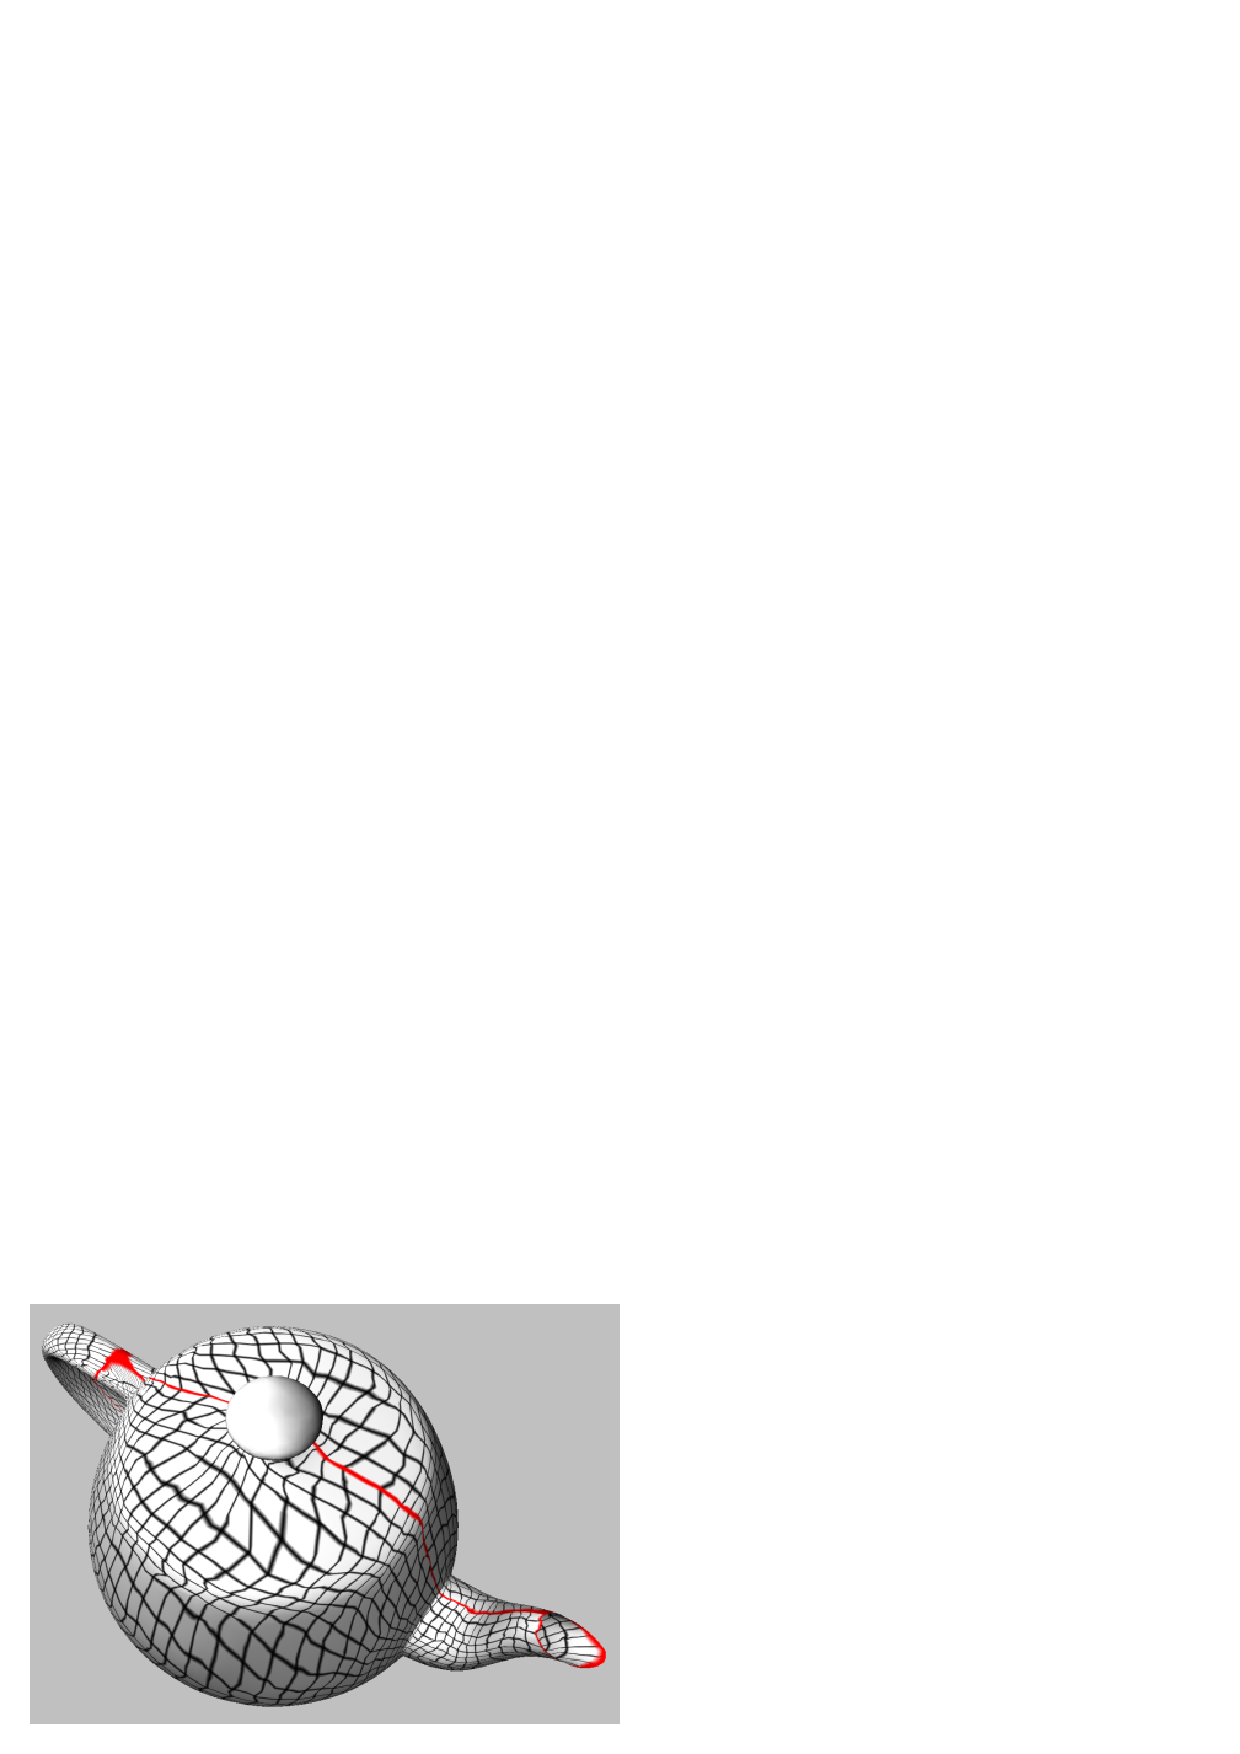
\includegraphics[width=1.0\textwidth]{Surface_mesh_parameterization/uniform}
    \end{ccTexOnly}
    \begin{ccHtmlOnly}
        <img width="90%" border=0 src="./uniform.png"><P>
    \end{ccHtmlOnly}
    % Title
    \begin{figure}[h]
        \caption{Left: Tutte barycentric mapping parameterization (the red
                 line depicts the cut graph). Right: parameter space.}
    \end{figure}
\end{center}


\subsubsection{Discrete Conformal Map}

\ccc{CGAL::Discrete_conformal_map_parameterizer_3<ParameterizationMesh_3, BorderParameterizer_3, SparseLinearAlgebraTraits_d>}  \\

Discrete conformal map parameterization has been introduced by Eck et
al. to the graphics community~\cite{cgal:eddhls-maam-95}. It attempts to
lower angle deformation by minimizing a discrete version of the
Dirichlet energy as derived by Pinkall and
Polthier~\cite{cgal:pp-cdmsc-93}. A one-to-one mapping is guaranteed
only when the two following conditions are fulfilled: the barycentric mapping condition (each vertex in parameter space is a convex combination if
its neighboring vertices), and the border is convex. This method solves two \#vertices x \#vertices sparse linear
systems. The matrix (the same for both systems) is sparse and symmetric definite
positive, thus can be efficiently solved using dedicated linear
solvers.

% Discrete conformal map
\begin{center}
    \label{Surface_mesh_parameterization-fig-conformal}
    % Image
    \begin{ccTexOnly}
        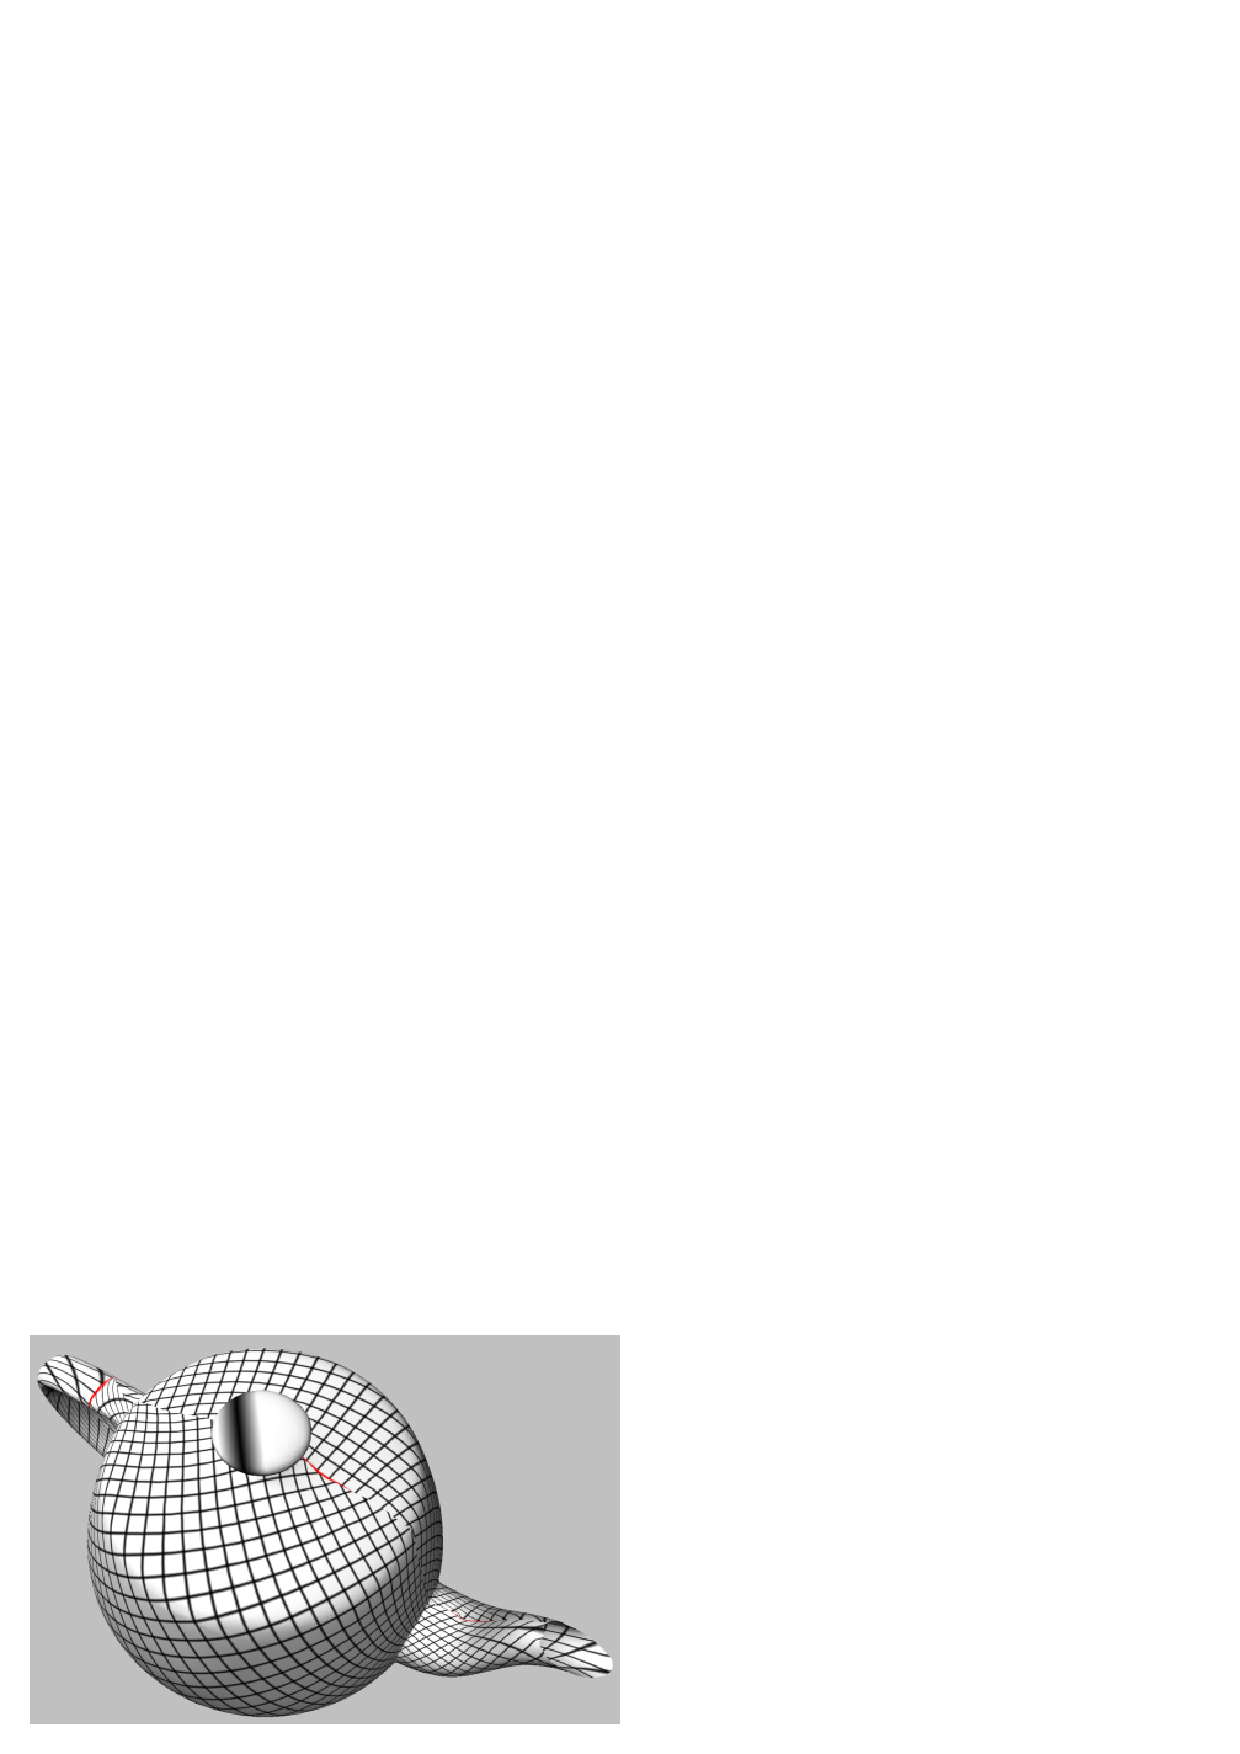
\includegraphics[width=0.45\textwidth]{Surface_mesh_parameterization/conformal}
    \end{ccTexOnly}
    \begin{ccHtmlOnly}
        <img width="90%" border=0 src="./conformal.png"><P>
    \end{ccHtmlOnly}
    % Title
    \begin{figure}[h]
        \caption{Left: discrete conformal map. Right: parameter space.}
    \end{figure}
\end{center}

\subsubsection{Floater Mean Value Coordinates}

\ccc{CGAL::Mean_value_coordinates_parameterizer_3<ParameterizationMesh_3, BorderParameterizer_3, SparseLinearAlgebraTraits_d>}  \\

The mean value coordinates parameterization method has been introduced
by Floater~\cite{cgal:f-mvc-03}. Each vertex in parameter space is
optimized so as to be a convex combination of its neighboring
vertices. The barycentric coordinates are this time unconditionally
positive, by deriving an application of the mean theorem for harmonic
functions. This method is in essence an approximation of the discrete conformal
maps, with a guaranteed one-to-one mapping when the border is convex. This method solves two \#vertices x \#vertices sparse linear systems. The matrix (the
same for both systems) is asymmetric.

% Floater mean value coordinates
\begin{center}
    \label{Surface_mesh_parameterization-fig-floater}
    % Image
    \begin{ccTexOnly}
      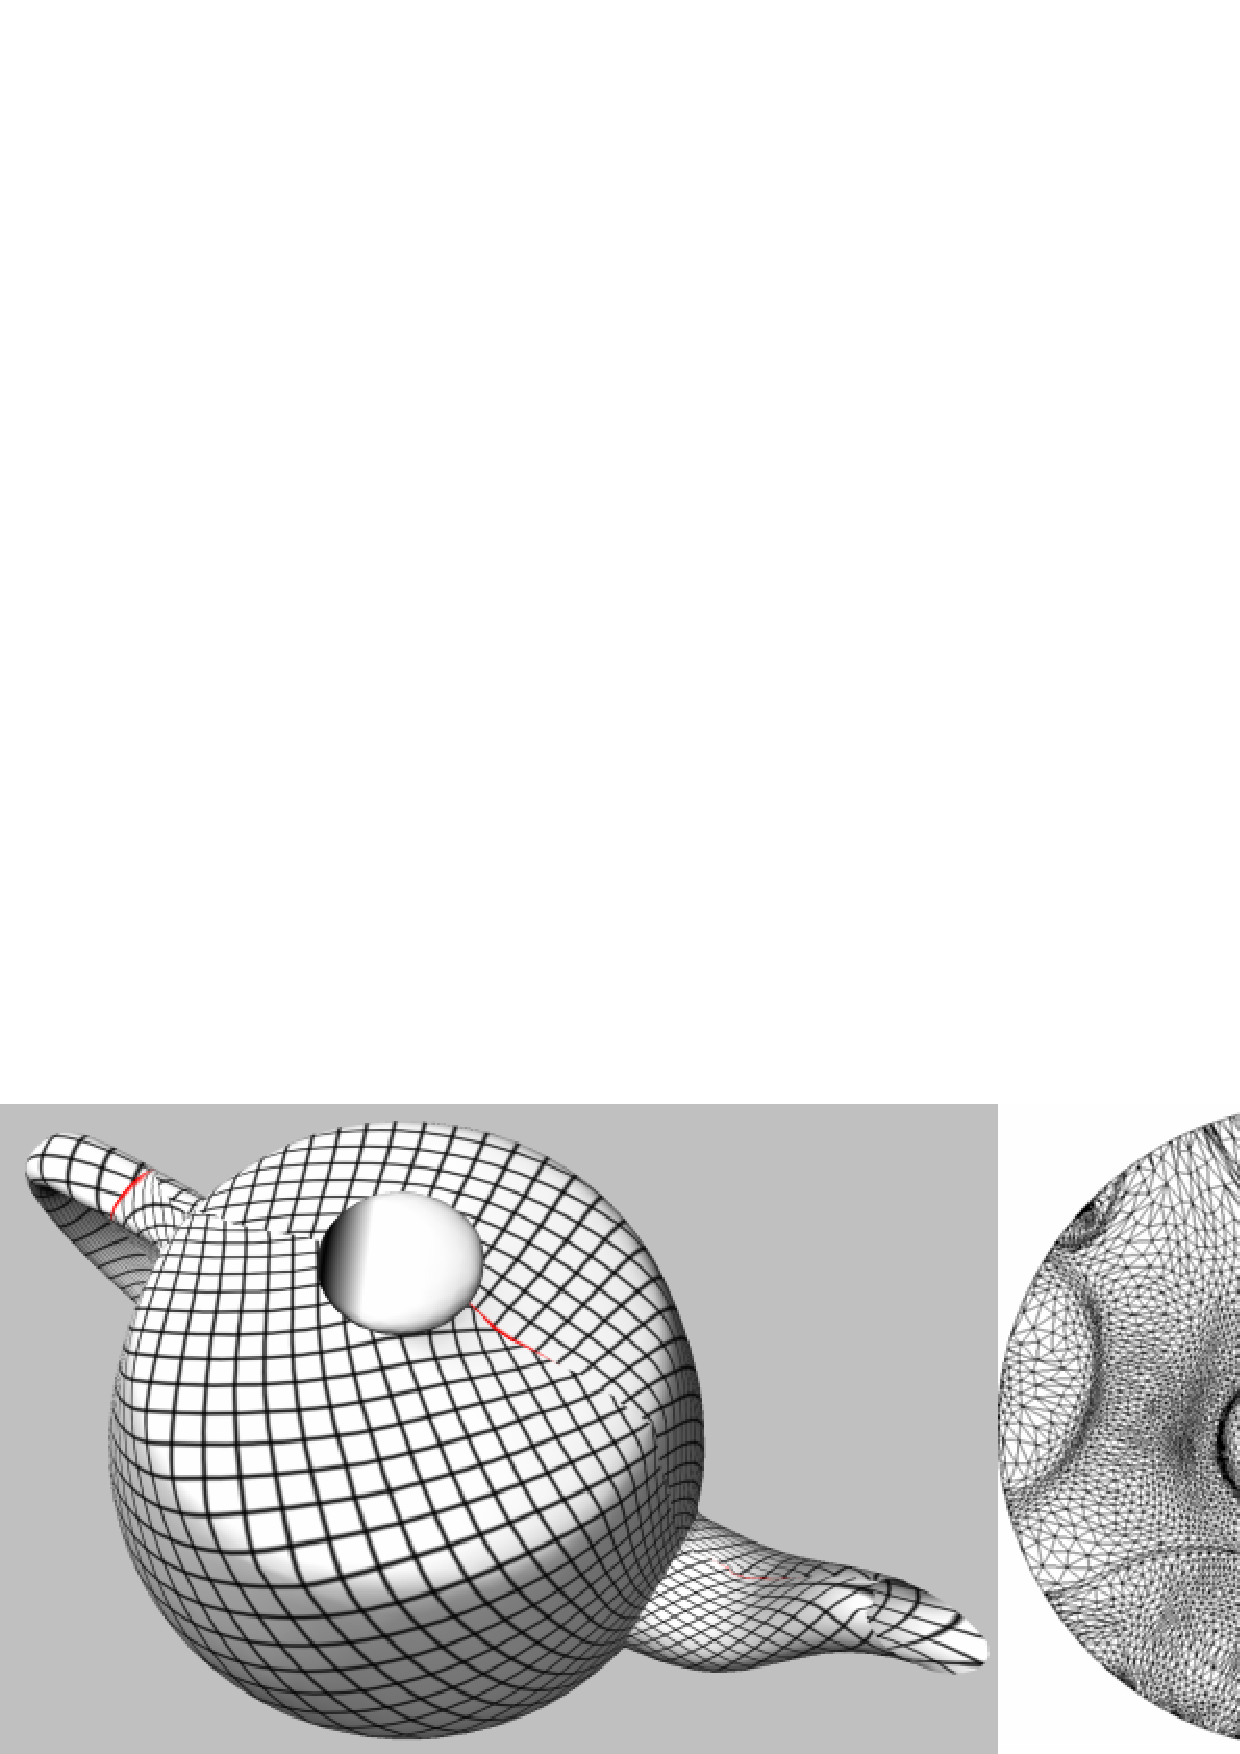
\includegraphics[width=1.0\textwidth]{Surface_mesh_parameterization/floater}
    \end{ccTexOnly}
    \begin{ccHtmlOnly}
        <img width="90%" border=0 src="./floater.png"><P>
    \end{ccHtmlOnly}
    % Title
    \begin{figure}[h]
        \caption{Floater Mean Value Coordinates}
    \end{figure}
\end{center}

\subsubsection{Discrete Authalic parameterization}

\ccc{CGAL::Discrete_authalic_parameterizer_3<ParameterizationMesh_3, BorderParameterizer_3, SparseLinearAlgebraTraits_d>}  \\

The discrete authalic parameterization method has been introduced by
Desbrun et al.~\cite{cgal:dma-ipsm-02}. It corresponds to
a weak formulation of an area-preserving method, and in essence
locally minimizes the area distortion. A one-to-one mapping is
guaranteed only if the convex combination condition is fulfilled and
the border is convex. This method solves two
\#vertices x \#vertices sparse linear systems. The matrix (the same
for both systems) is asymmetric.

% Discrete authalic parameterization
\begin{center}
    \label{Surface_mesh_parameterization-fig-authalic}
    % Image
    \begin{ccTexOnly}
        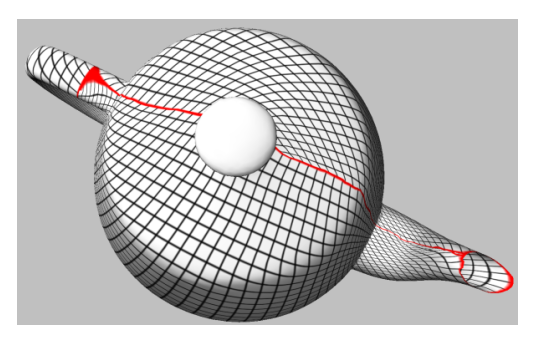
\includegraphics[width=1.0\textwidth]{Surface_mesh_parameterization/authalic}
    \end{ccTexOnly}
    \begin{ccHtmlOnly}
        <img width="90%" border=0 src="./authalic.png"><P>
    \end{ccHtmlOnly}
    % Title
    \begin{figure}[h]
        \caption{Discrete Authalic Parameterization}
    \end{figure}
\end{center}

\subsubsection{Border Parameterizations for Fixed Methods}
\label{sec:Border-Parameterizations-for-Fixed-Methods}

Parameterization methods for
borders are used as traits classes modifying the behavior of
\ccc{ParameterizerTraits_3} models.
They are provided as models of the \ccc{BorderParameterizer_3} concept. Border parameterizations for fixed border surface parameterizations
are a family of methods to define a set of constraints, namely two
$u,v$ coordinates for each vertex along the border.

\begin{itemize}

\item
    The user can select a border parameterization among
    two commonly used methods: uniform or arc-length parameterization.

    \emph{Usage:}

    Uniform border parameterization is more stable, although it gives
    poor visual results. The
    arc-length border parameterization is used by default.

\item
    One convex shape specified by one shape among two standard ones:
    a circle or a square.

    \emph{Usage:}

    The circular border parameterization is used by default as it
    corresponds to the simplest convex shape. The square border
    parameterization is commonly used for texture mapping.

\end{itemize}

\ccc{CGAL::Circular_border_arc_length_parameterizer_3<ParameterizationMesh_3>}  \\
\ccc{CGAL::Circular_border_uniform_parameterizer_3<ParameterizationMesh_3>}  \\
\ccc{CGAL::Square_border_arc_length_parameterizer_3<ParameterizationMesh_3>}  \\
\ccc{CGAL::Square_border_uniform_parameterizer_3<ParameterizationMesh_3>}  \\

% Julius Cesar mask circular vs square border
\begin{center}
    \label{Surface_mesh_parameterization-fig-circular_border}
    % Image
    \begin{ccTexOnly}
        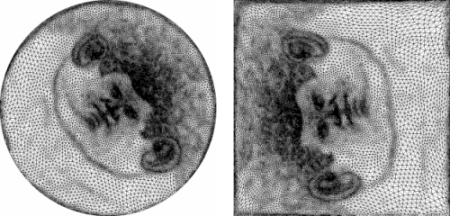
\includegraphics[width=0.80\textwidth]{Surface_mesh_parameterization/border}
    \end{ccTexOnly}
    \begin{ccHtmlOnly}
        <img width="80%" border=0 src="./border.png"><P>
    \end{ccHtmlOnly}
    % Title
    \begin{figure}[h]
        \caption{Left: Julius Cesar mask parameterization with
                 Authalic/circular border. Right: Julius Cesar mask's
                 image with Floater/square border.}
    \end{figure}
\end{center}



\subsection{Free Border Surface Parameterizations}

\subsubsection{Least Squares Conformal Maps}

\ccc{CGAL::LSCM_parameterizer_3<ParameterizationMesh_3, BorderParameterizer_3, SparseLinearAlgebraTraits_d>}  \\

The Least Squares Conformal Maps (LSCM) parameterization method has
been introduced by L\'evy et al.~\cite{cgal:lprm-lscm-02}. It corresponds to a conformal method with a free border (at least two
vertices have to be constrained to obtain a unique solution), which
allows further lowering of the angle distortion. A one-to-one mapping
is not guaranteed by this method. It solves a (2 $\times$
\#triangles) $\times$ \#vertices sparse linear system in the least squares sense,
which implies solving a symmetric matrix.

% LSCM
\begin{center}
    \label{Surface_mesh_parameterization-fig-LSCM}
    % Image
    \begin{ccTexOnly}
        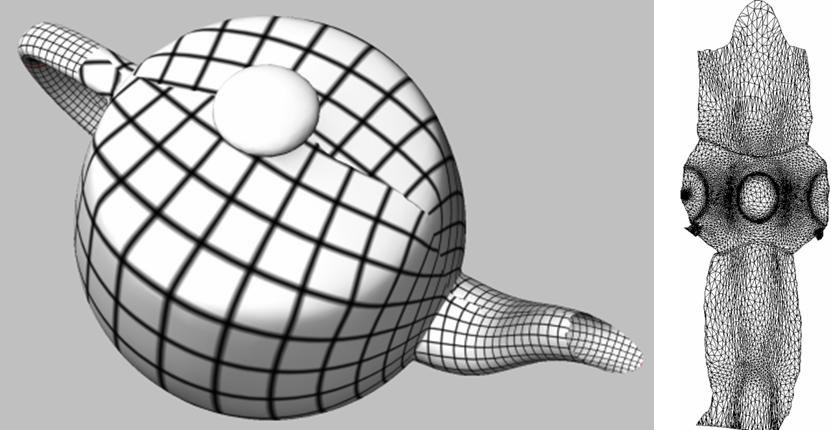
\includegraphics[width=1.0\textwidth]{Surface_mesh_parameterization/LSCM}
    \end{ccTexOnly}
    \begin{ccHtmlOnly}
        <img width="90%" border=0 src="./LSCM.png"><P>
    \end{ccHtmlOnly}
    % Title
    \begin{figure}[h]
        \caption{Least squares conformal maps.}
    \end{figure}
\end{center}


\subsubsection{Border Parameterizations for Free Methods}
\label{sec:Border-Parameterizations-for-Free-Methods}

Parameterization methods for
borders are used as traits classes modifying the behavior of
\ccc{ParameterizerTraits_3} models. They are provided as models of the \ccc{BorderParameterizer_3} concept.
The border parameterizations associated to free border surface
parameterization methods define only two constraints: the pinned vertices.

\begin{itemize}

\item
    \ccc{CGAL::Two_vertices_parameterizer_3<ParameterizationMesh_3>}  \\

    \emph{Usage:}

    \ccc{CGAL::Two_vertices_parameterizer_3<ParameterizationMesh_3>} is the default
    free border parameterization, and is the only one available
    in the current version of this package.

\end{itemize}


\subsection{Discrete Authalic Parameterization Example}

\ccc{Authalic_parameterization.C} computes a Discrete Authalic parameterization
over a \ccc{CGAL::Polyhedron_3<Traits>} mesh. Specifying a specific surface parameterization instead of the default one means using the second parameter of \ccc{CGAL::parameterize()}. The differences with the first example \ccc{Simple_parameterization.C} are:

\begin{ccExampleCode}

#include <CGAL/Discrete_authalic_parameterizer_3.h>

...

//***************************************
// Discrete Authalic Parameterization
//***************************************

typedef CGAL::Discrete_authalic_parameterizer_3<Parameterization_polyhedron_adaptor>
                                                    Parameterizer;

Parameterizer::Error_code err = CGAL::parameterize(mesh_adaptor, Parameterizer());

...

\end{ccExampleCode}


\subsection{Square Border Arc Length Parameterization Example}

\ccc{Square_border_parameterization.C} computes a Floater mean value coordinates
parameterization with a square border arc length parameterization.
Specifying a specific border parameterization
instead of the default one means using the second parameter of
\ccc{CGAL::Mean_value_coordinates_parameterizer_3<ParameterizationMesh_3, BorderParameterizer_3, SparseLinearAlgebraTraits_d>}. The differences with the first example \ccc{Simple_parameterization.C} are:

\begin{ccExampleCode}

#include <CGAL/Square_border_parameterizer_3.h>

...

//***************************************
// Floater Mean Value Coordinates parameterization
// with square border
//***************************************

// Square border parameterizer
typedef CGAL::Square_border_arc_length_parameterizer_3<Parameterization_polyhedron_adaptor>
                                                        Border_parameterizer;

// Floater Mean Value Coordinates parameterizer with square border
typedef CGAL::Mean_value_coordinates_parameterizer_3<Parameterization_polyhedron_adaptor,
                                                        Border_parameterizer>
                                                    Parameterizer;

Parameterizer::Error_code err = CGAL::parameterize(mesh_adaptor, Parameterizer());

...

\end{ccExampleCode}

